\section{从 UML 图到代码}

每种 UML 元素只对应一种写法，规则先定下，后面逐类翻译即可（\tabref{tab:mapping}）。

\begin{table}[htbp]
\centering
\caption{UML 元素到 Python 构造的转换规则}\label{tab:mapping}
\zihao{-5}
\renewcommand{\arraystretch}{1.2}
\begin{tabularx}{\textwidth}{@{}L{2.5cm}L{4.3cm}Y@{}}
\toprule
UML 元素 & 代码构造 & 处理要点 \\
\midrule
类（实体） & \code{@dataclass} & 字段照抄；主键统一暴露 \code{ident} \\
枚举 & \code{class X(str, Enum)} & 便于 JSON 落盘与按名字解析 \\
关联（1—N） & 外键字段 + 仓储查询 & 不挂对象引用，避免循环引用 \\
组合（Item—ItemRevision） & 独立表 + 按 \code{itemId} 查 & 待审内容能被单独丢弃 \\
操作（方法） & 服务层方法 & 跨聚合读写放服务层 \\
状态图 & 迁移表 + \code{apply\_status} & 每条箭头一个表项 \\
时序图 & 一个方法体 + 锁 & \code{alt} 分支即 \code{if/else} \\
\bottomrule
\end{tabularx}
\end{table}

\subsection{类图}

领域模型（\figref{fig:class}）照实验二类图逐类翻译，10 个实体加 5 个枚举落在 \code{models.py}。实体只保留自身判断，跨实体协作放服务层。\code{ItemRevision} 是组合状态载体：已发布商品被修改时 \code{Item.status} 仍为已发布，新内容暂存于待审记录，审核通过后原子替换。\code{Reservation.requestId} 是幂等键。

\begin{figure}[!htbp]
\centering
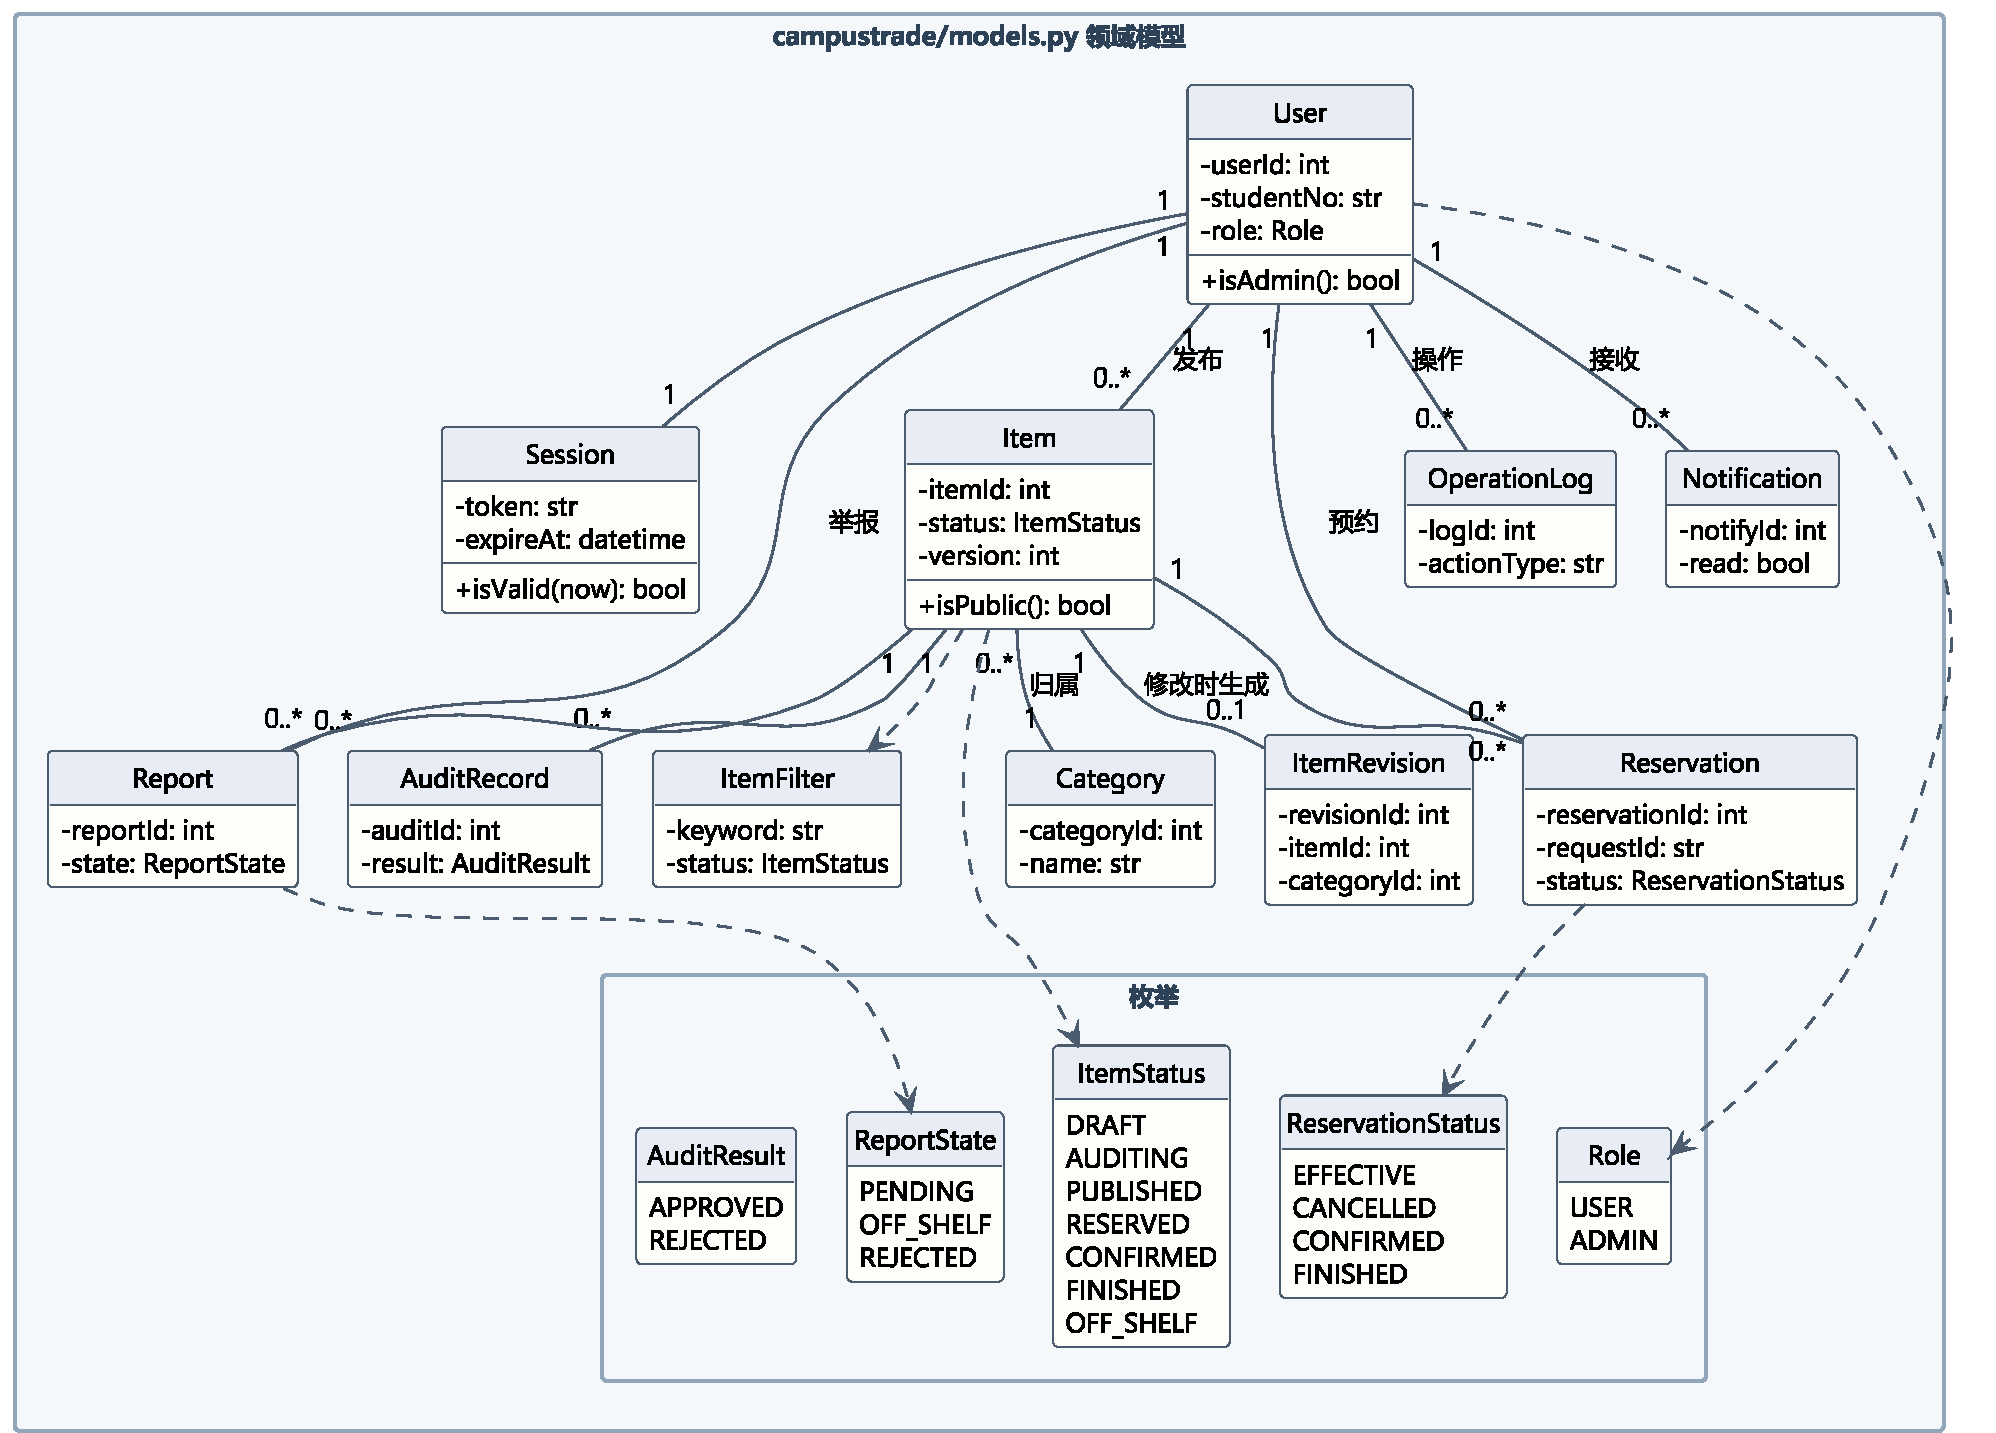
\includegraphics[width=\textwidth]{class.pdf}
\caption{领域模型类图}\label{fig:class}
\end{figure}

服务层与仓储（\figref{fig:service}）是实现期新增：\code{ServiceBase} 收敛令牌换用户与落盘，六个业务服务继承它；\code{Store} 是仓储门面，\code{Table} 是泛型内存表。

\begin{figure}[!htbp]
\centering
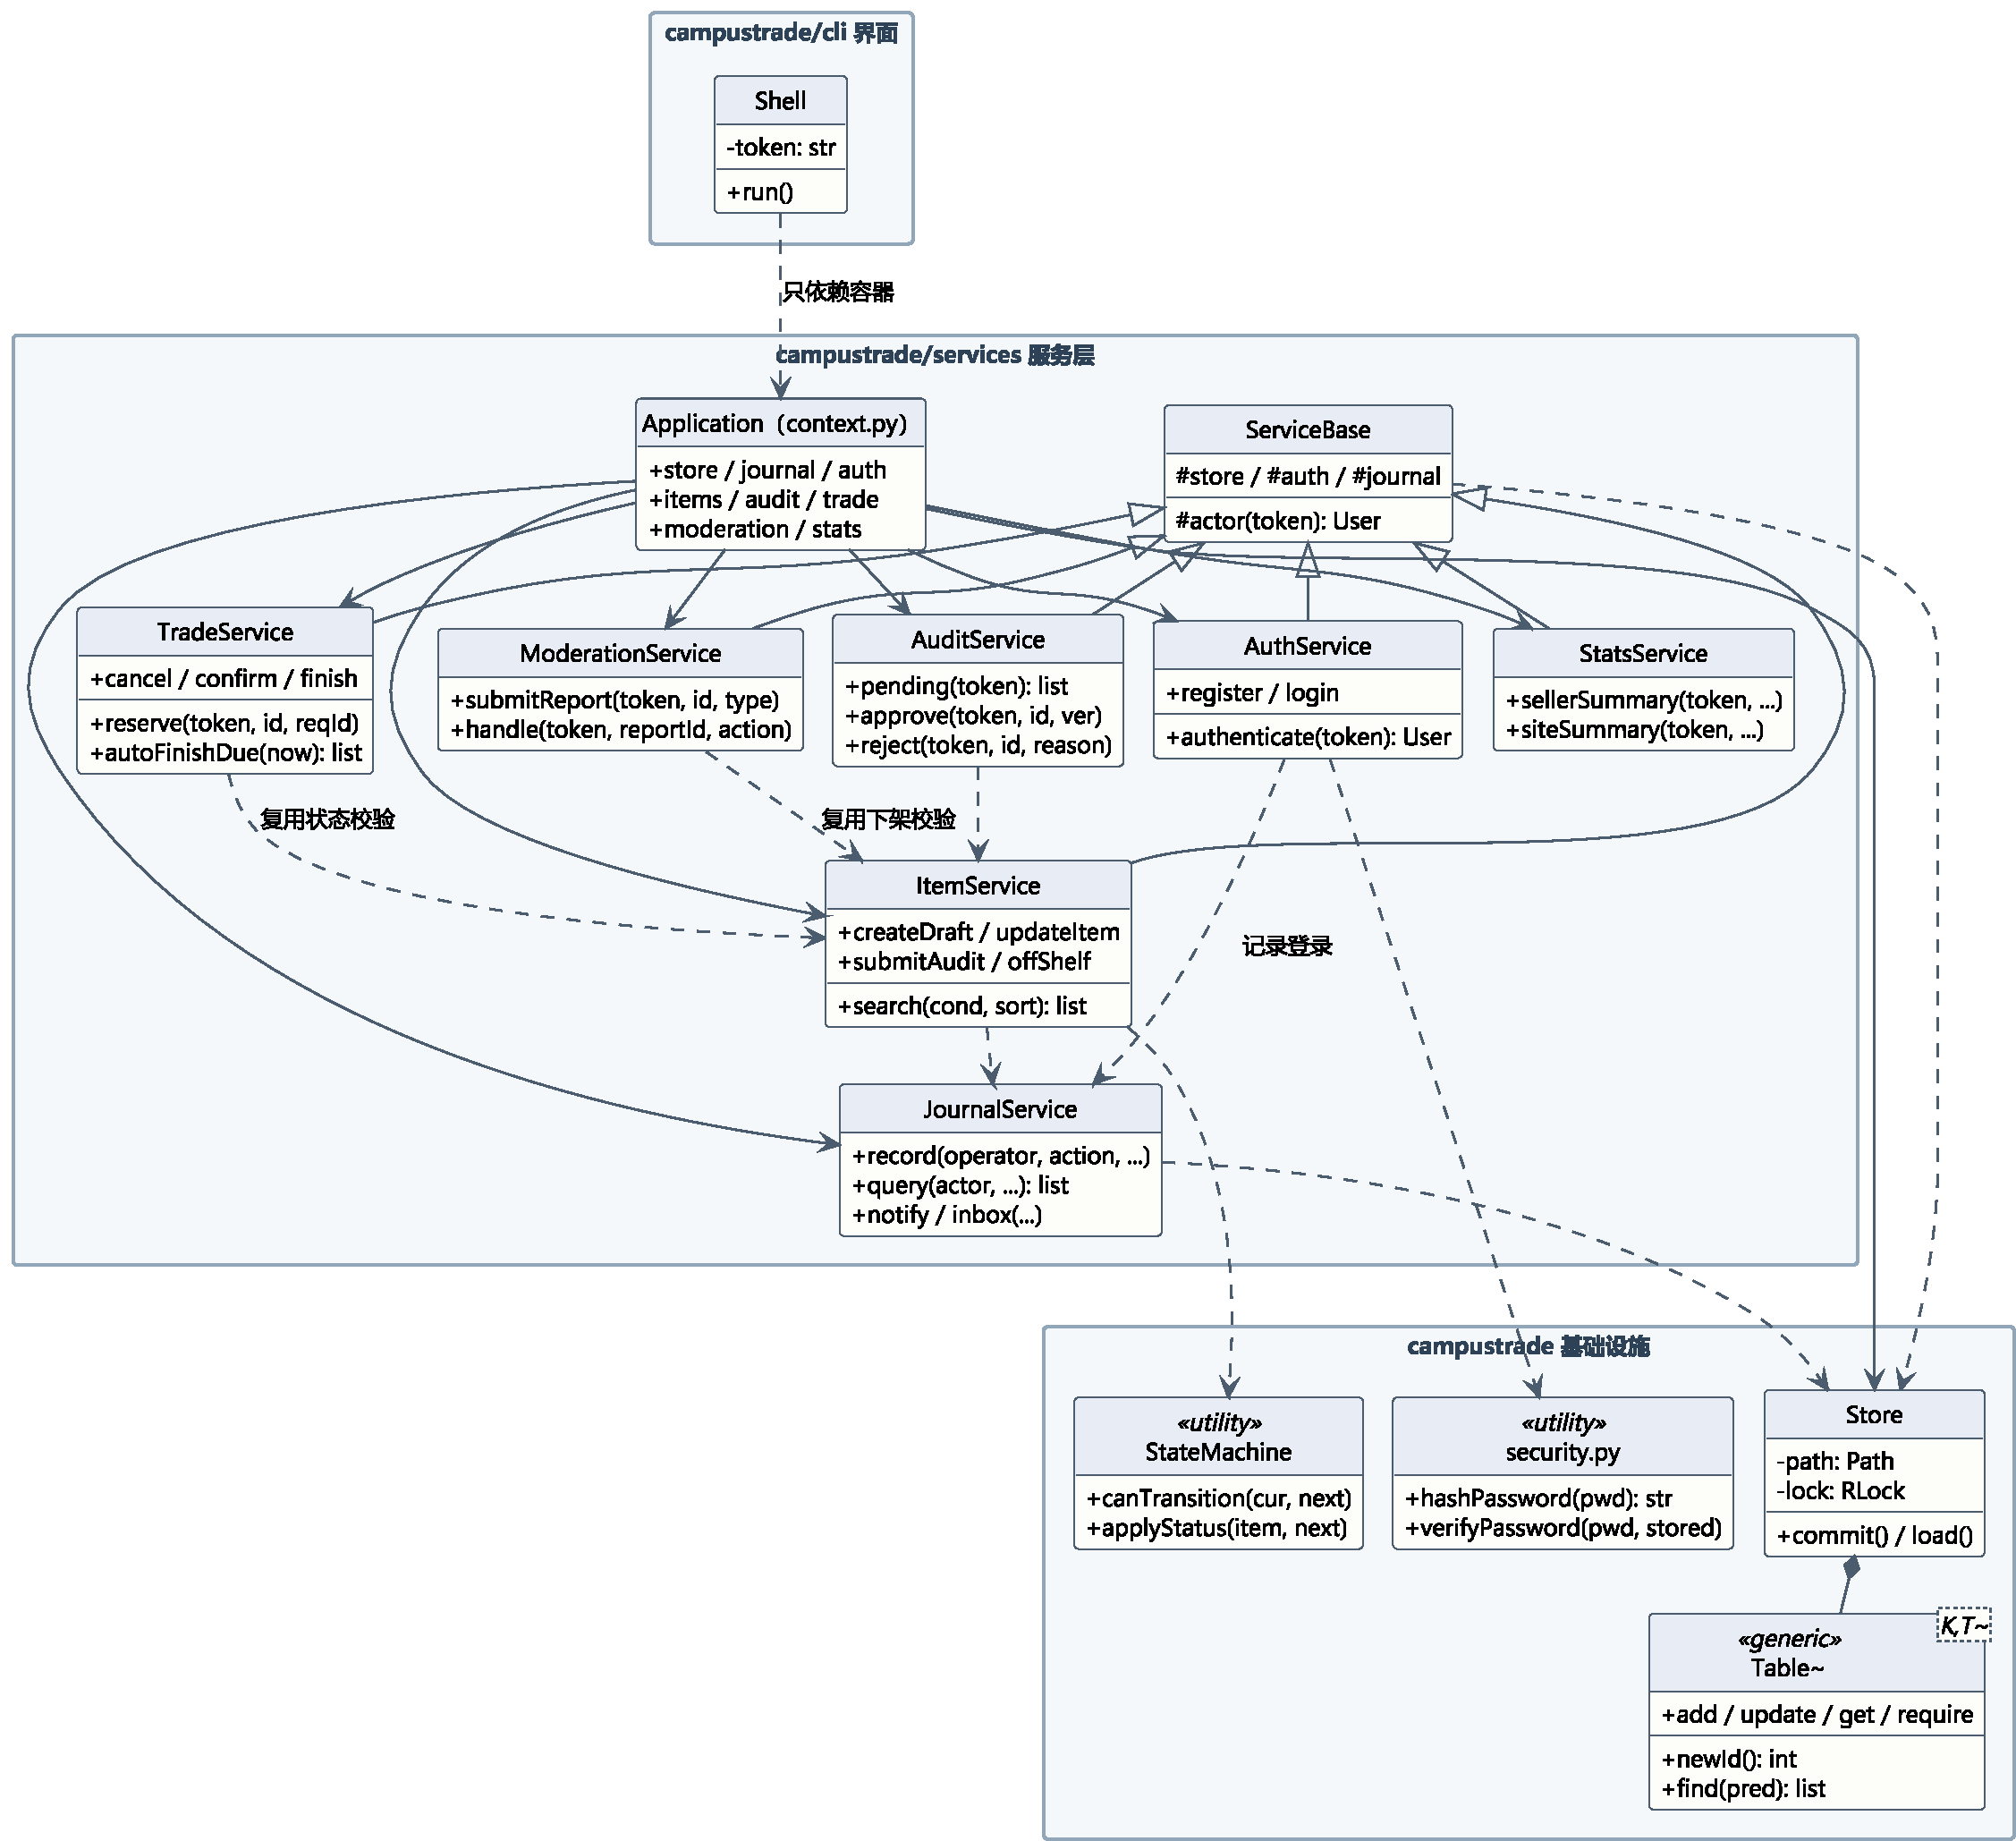
\includegraphics[width=0.82\textwidth]{service.pdf}
\caption{服务层与仓储类图}\label{fig:service}
\end{figure}

实现时对原设计改了三处：一是实体上的业务方法上移到服务层（方法需跨聚合读写，实体会被迫持有仓储引用，事务边界不清）；二是 \code{ItemRevision} 增加 \code{categoryId}（改分类也属修改商品信息，不带分类会导致审核后内容与分类不一致）；三是新增 \code{ServiceBase}、\code{Store}、\code{Table} 三个工程类，收敛重复代码。

\subsection{状态图}

7 个状态、9 条合法迁移写成 \code{state.py} 里的一个字典，\code{apply\_status()} 先校验再赋值并递增 \code{version}（\figref{fig:state}、\tabref{tab:transition}）。非法迁移一律抛 \code{Conflict}。

\begin{figure}[!htbp]
\centering
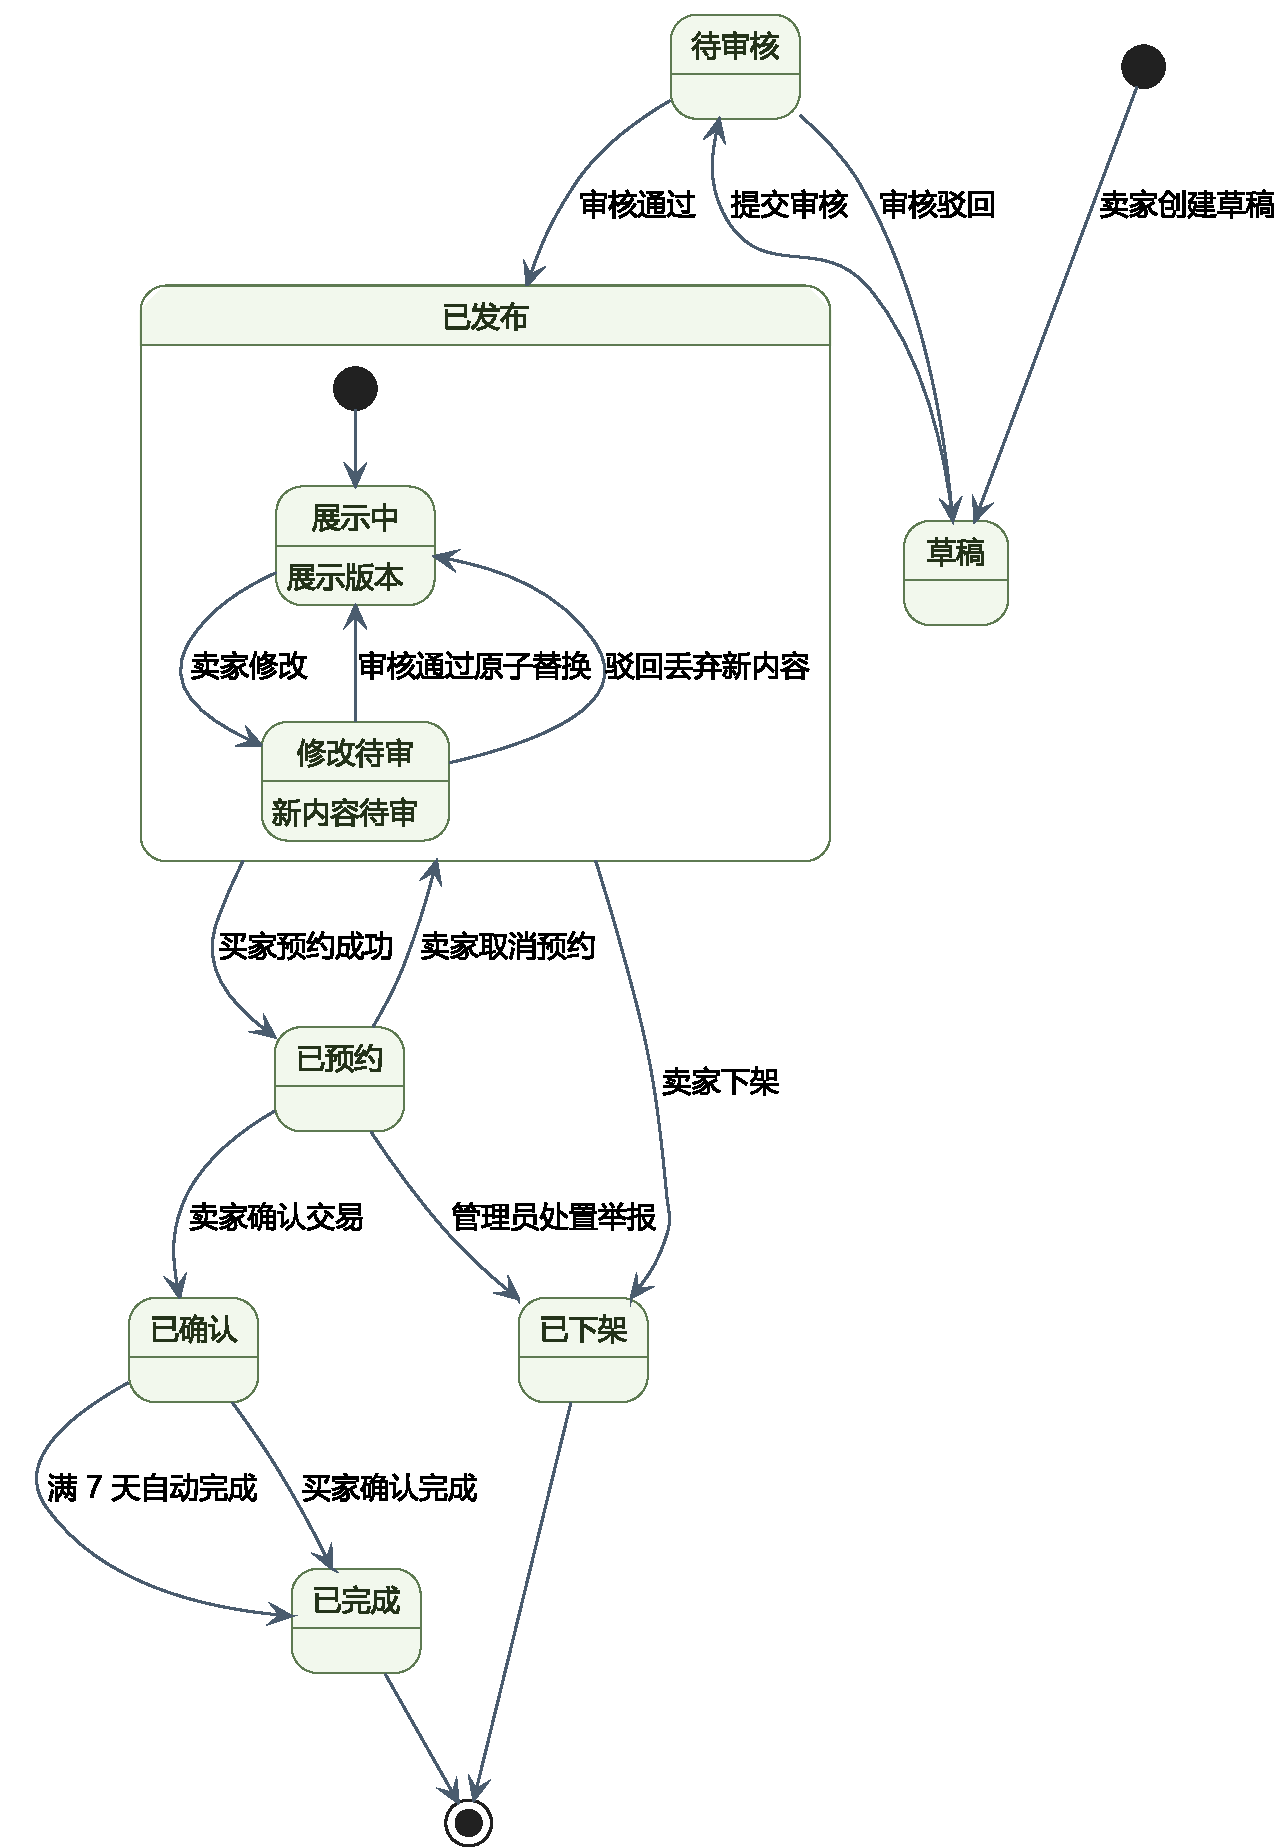
\includegraphics[width=0.29\textwidth]{state.pdf}
\caption{商品状态图}\label{fig:state}
\end{figure}

\begin{table}[htbp]
\centering
\caption{状态迁移与触发动作}\label{tab:transition}
\zihao{-5}
\renewcommand{\arraystretch}{1.15}
\begin{tabularx}{\textwidth}{@{}L{3.3cm}L{4.3cm}Y@{}}
\toprule
迁移 & 触发方法 & 附加校验 \\
\midrule
草稿 $\to$ 待审核 & \code{ItemService.submit\_audit} & 必填字段；仅本人 \\
待审核 $\to$ 已发布 & \code{AuditService.approve} & 仅管理员；版本比对 \\
待审核 $\to$ 草稿 & \code{AuditService.reject} & 必填驳回原因 \\
已发布 $\to$ 已预约 & \code{TradeService.reserve} & 锁内查重；幂等键 \\
已预约 $\to$ 已发布 & \code{TradeService.cancel} & 仅卖家 \\
已预约 $\to$ 已确认 & \code{TradeService.confirm} & 仅卖家 \\
已确认 $\to$ 已完成 & \code{TradeService.finish} & 仅预约买家；满 7 天自动完成 \\
已发布 $\to$ 已下架 & \code{ItemService.off\_shelf} & 仅本人或管理员 \\
已下架 $\to$ 已发布 & \code{ItemService.restore} & 仅管理员 \\
\bottomrule
\end{tabularx}
\end{table}

\subsection{时序图}

预约流程按\figref{fig:seq}逐条翻译，\code{alt} 分支对应 \code{raise}，\code{with store.lock} 对应临界区。查重放在最前，重发请求此时商品已是已预约，若先校验状态会把重发误判为冲突。

\begin{figure}[!htbp]
\centering
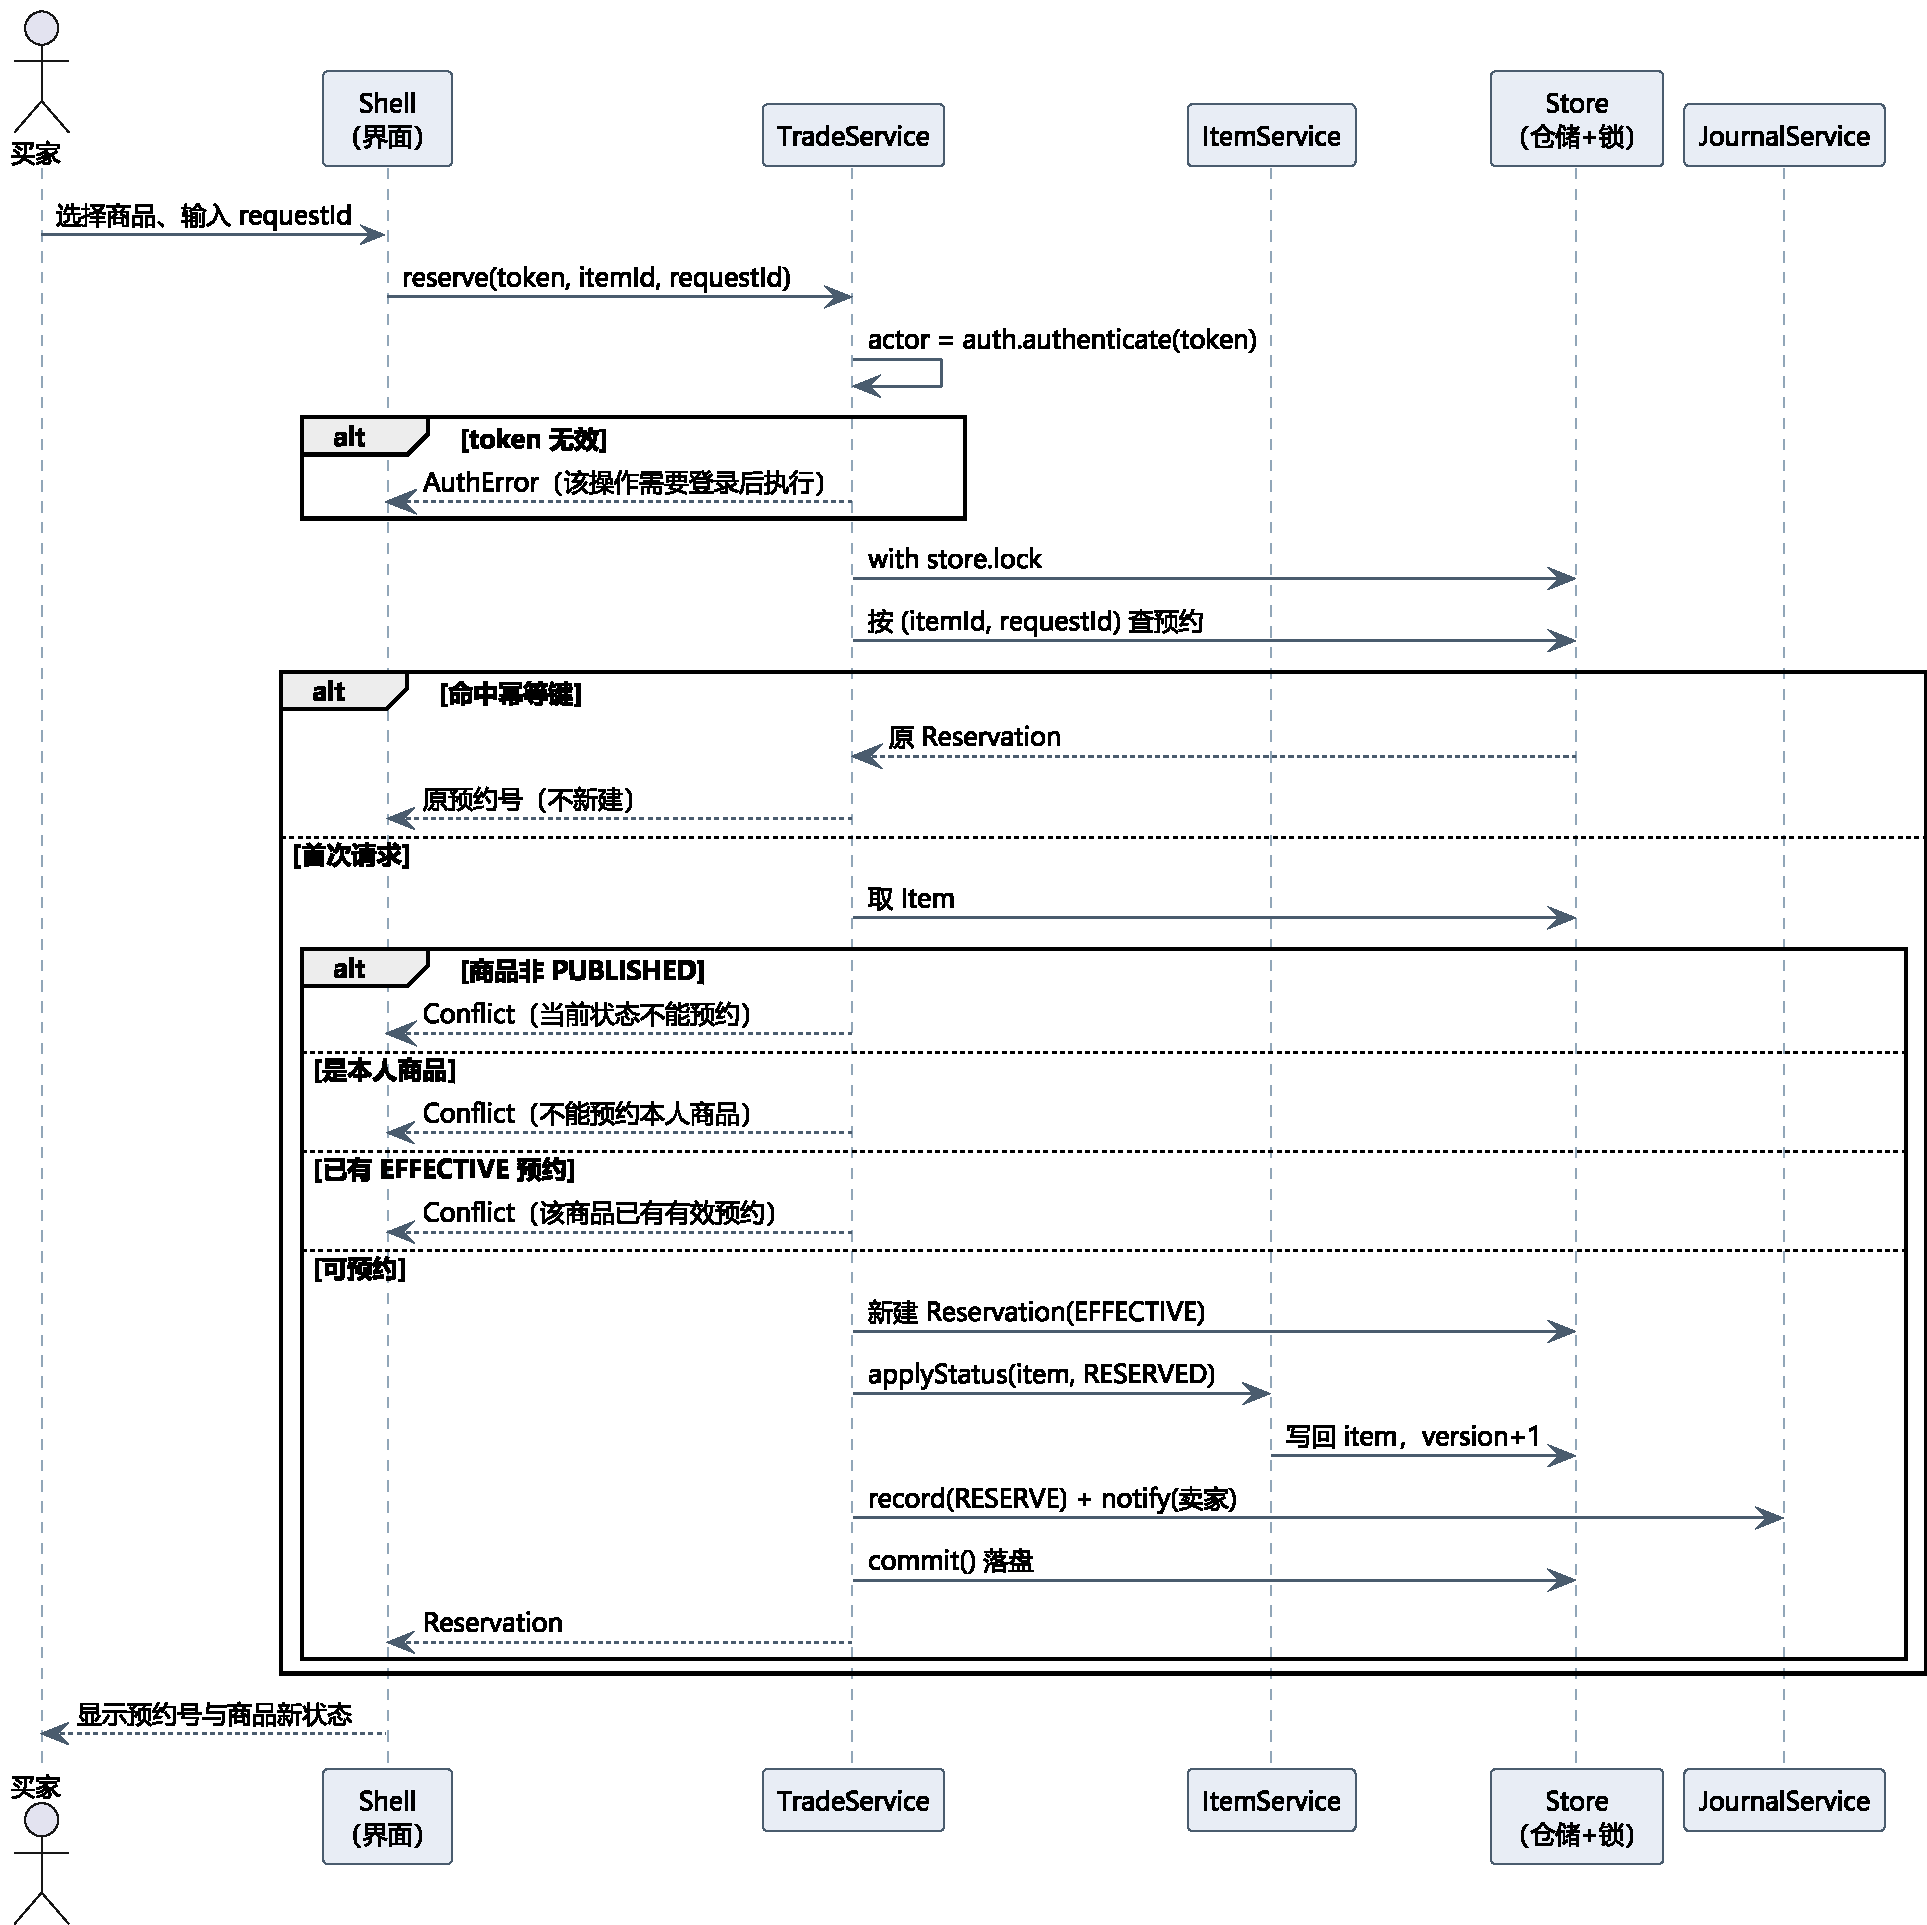
\includegraphics[width=0.74\textwidth]{seq_reserve.pdf}
\caption{预约商品时序图}\label{fig:seq}
\end{figure}

修改已发布商品（\figref{fig:seq2}）把待审内容与商品状态解耦：修改只写 \code{ItemRevision}，前台仍显示旧信息，审核期间买家照常预约；通过时原子替换全部字段，驳回则丢弃待审记录。

\begin{figure}[!htbp]
\centering
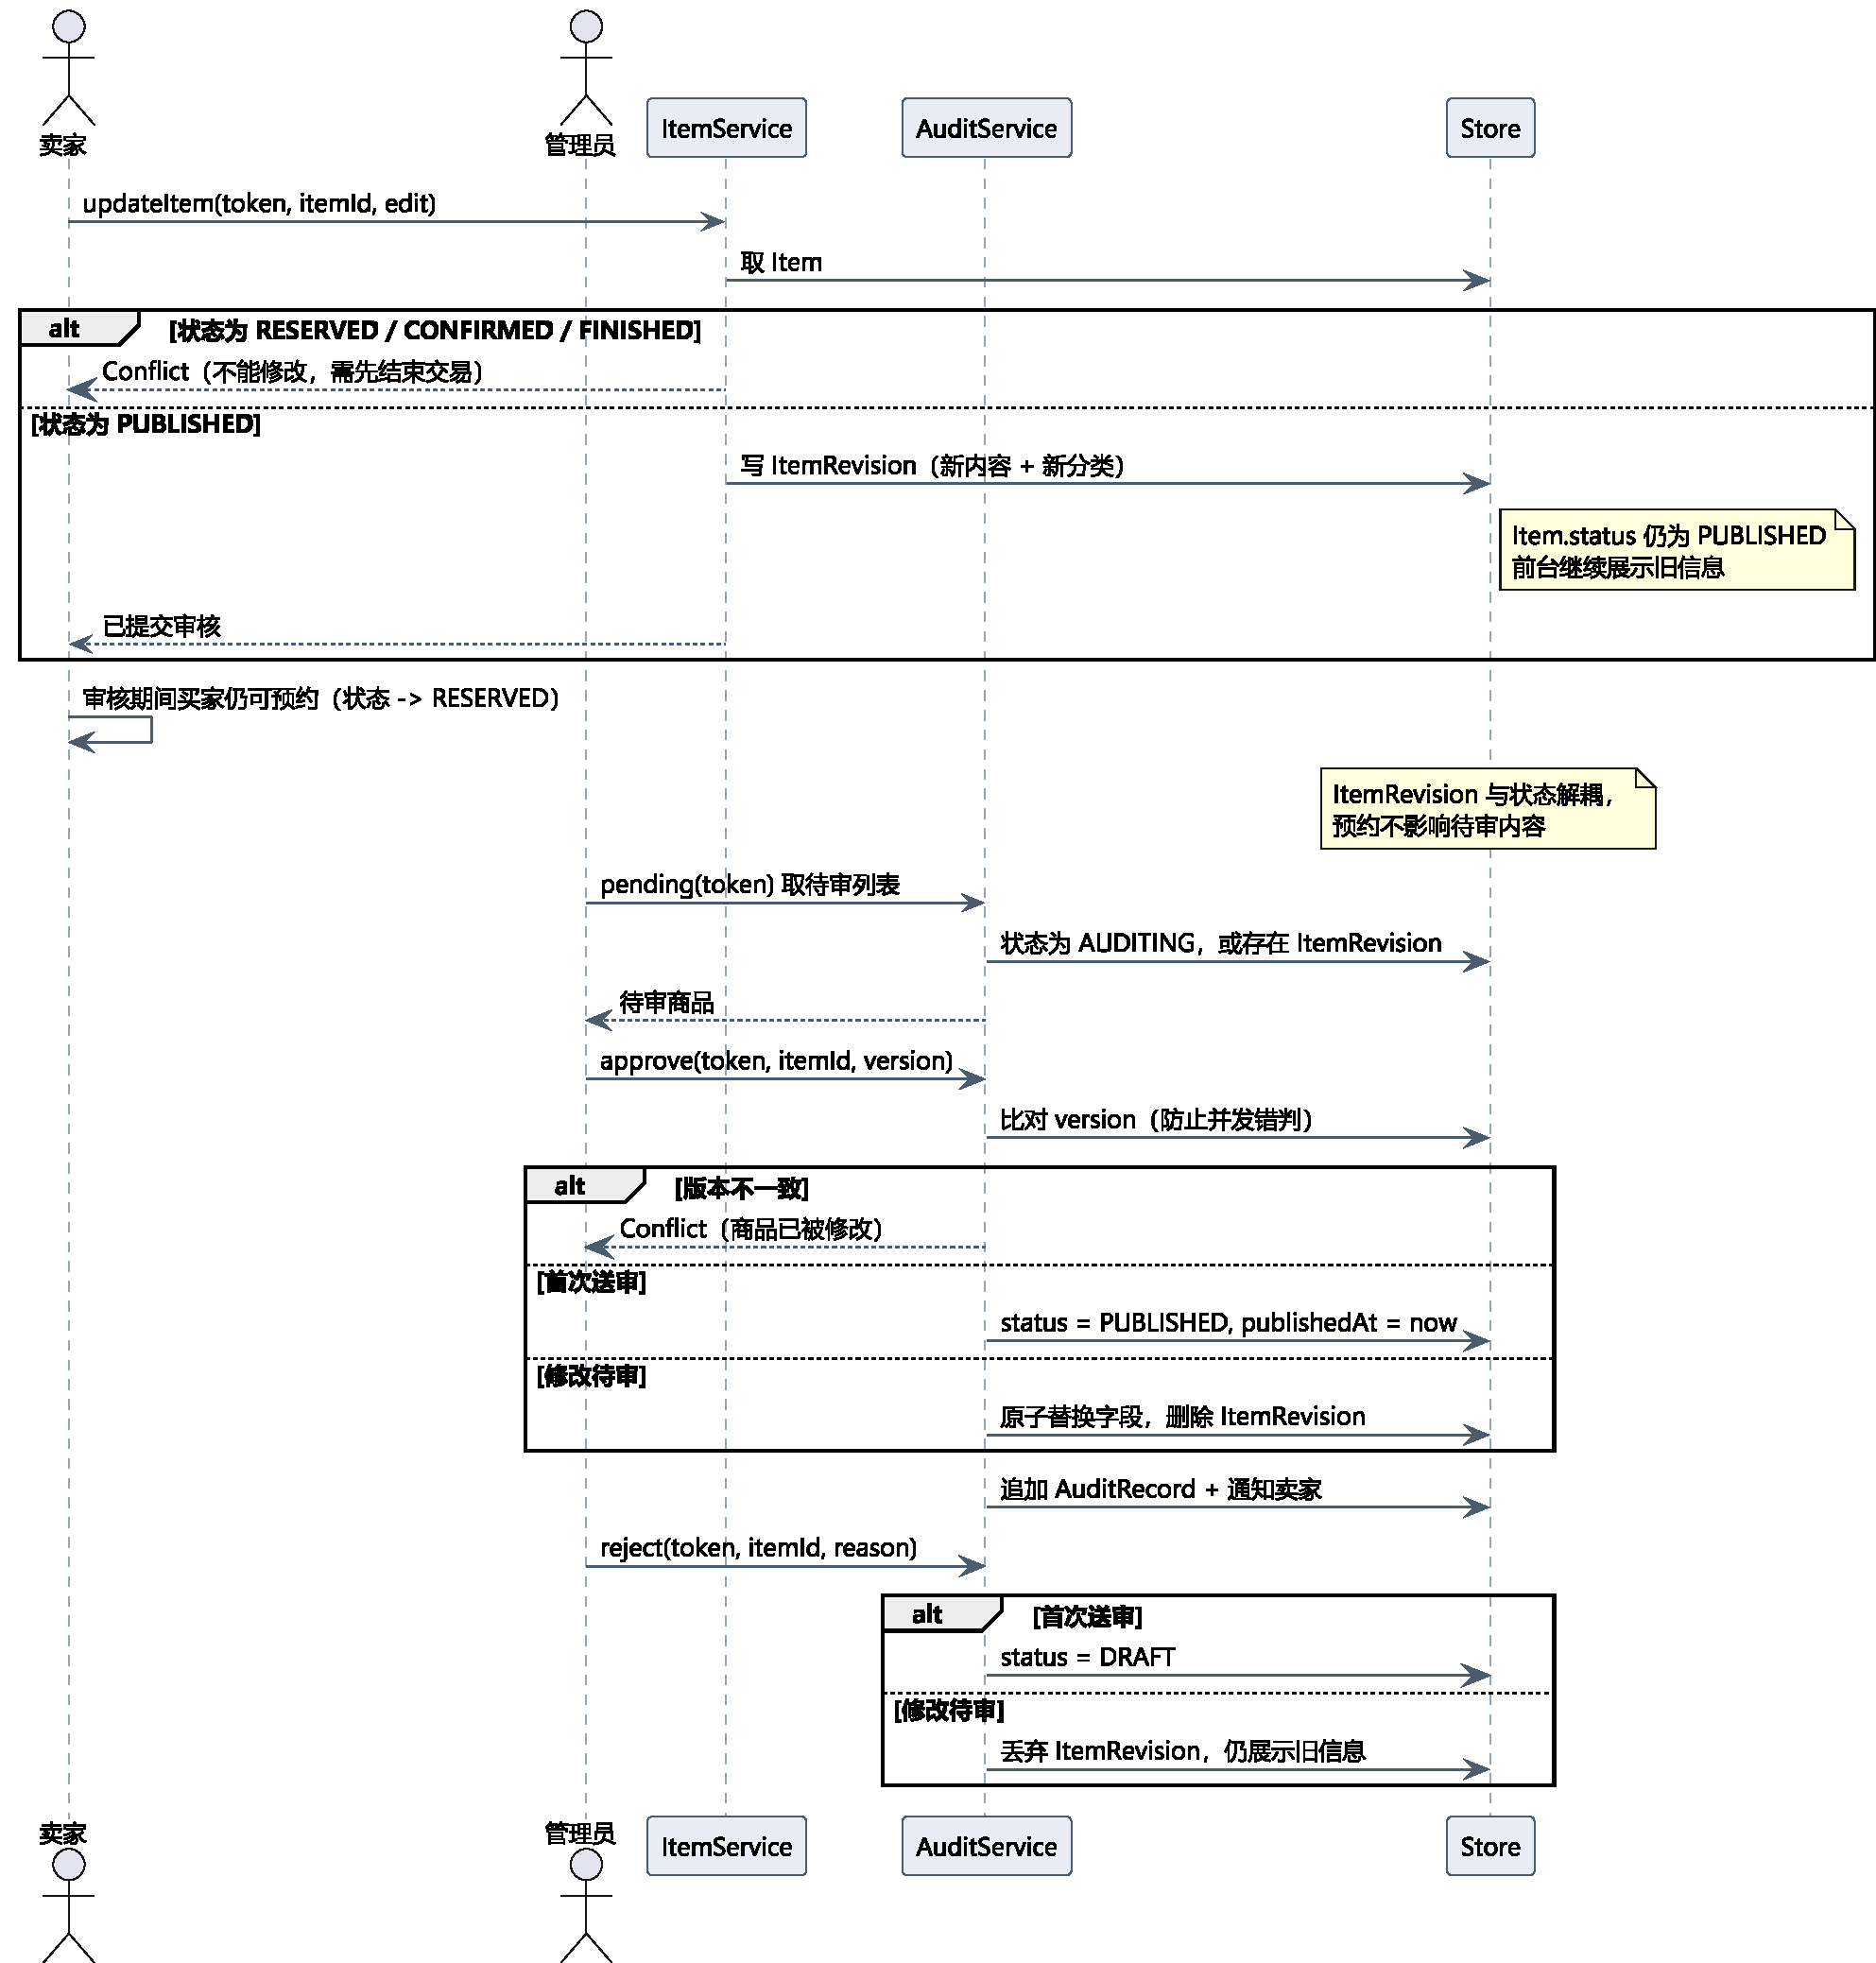
\includegraphics[width=0.7\textwidth]{seq_revision.pdf}
\caption{修改已发布商品与审核时序图}\label{fig:seq2}
\end{figure}

\subsection{代码规模}

共 22 个源文件、3311 行，去掉空行与注释后 \textbf{2761 行}；另有 8 个测试文件、73 个用例（\tabref{tab:loc}）。

\begin{table}[htbp]
\centering
\caption{源代码规模统计}\label{tab:loc}
\zihao{-5}
\renewcommand{\arraystretch}{1.18}
\begin{tabularx}{\textwidth}{@{}L{3.2cm}L{1.6cm}L{2.0cm}L{2.4cm}Y@{}}
\toprule
分组 & 文件数 & 总行数 & 有效代码行 & 主要文件 \\
\midrule
领域模型 & 3 & 513 & 377 & \code{models.py}（327） \\
基础设施 & 2 & 305 & 254 & \code{storage.py}（260） \\
服务层 & 9 & 1343 & 1186 & \code{item.py}（386）、\code{trade.py}（253） \\
界面层 & 3 & 602 & 500 & \code{shell.py}（530） \\
装配与入口 & 5 & 548 & 444 & \code{demo.py}（344） \\
\midrule
小计 & 22 & 3311 & \textbf{2761} & 平均每文件 126 行 \\
测试 & 8 & 794 & 577 & 73 个用例 \\
\bottomrule
\end{tabularx}
\end{table}
